\documentclass[a4paper,12pt,hidelinks]{report}

%%Pacchetti utili anche se non necessari

\usepackage{amsfonts}
\usepackage{amsmath}
\usepackage{latexsym}
\usepackage{tabularx}
\usepackage[italian]{babel}
\usepackage[bookmarks=true]{hyperref}
\usepackage{url}
% \usepackage{subfigure}
\usepackage{epstopdf}
\usepackage[utf8]{inputenc}
% \usepackage[utf8x]{inputenc}
\usepackage{listings}
\usepackage{graphicx}
\usepackage{color}

\usepackage{amsmath}


%-------------------------------------------

% \title{Progettazione sito web\\ ''B\&B La Vecchia Posta''}
% \author{Daniele Di Pompeo \\mat. 226766}
% \annoaccademico{2013-2014}
\begin{document}
  \begin{titlepage}
    \begin{center}
    % Upper part of the page
      
\includegraphics[width=0.5\textwidth,keepaspectratio=true]{../img/logo}\\[1cm]    
      \textsc{\LARGE Verifiche stile}\\[0.6cm]
      \textsc{\LARGE  progetto del sito:\\[0.5cm] ``B\&B La Vecchia Posta''}\\ [2.0cm]

    % Author and supervisor
      \begin{minipage}{0.8\textwidth}
	\begin{flushleft} \large
	  \emph{Autore:} Daniele Di Pompeo \\[0.5cm]
	  \emph{Versione documento: 1.0}\\[0.5cm]
	  \emph{Data emissione del documento: \today}\\[0.5cm]
	\end{flushleft}
      \end{minipage}
    \end{center}
  \end{titlepage}

% \tableofcontents
 
\begin{abstract}
Lo scopo del seguente documento è convalidare le scelte di scelte progettate differentemente. 
La prima parte descriverà la qualità grafica, successivamente verrà posta
l'attenzione per la compatibilità tra browser e in ultimo ma non meno importante si porrà l'attenzione sul rispetto dei requisiti per l'accessibilità per persone diversamente
abili.
\end{abstract}

\section*{Qualità della grafica}
Per valutare gli aspetti grafici si sono seguite le linee guide più classiche.
Gli oggetti cliccabili risultano essere tutti distinguibili grazie all'utilizzo di effetti di transizione grafica con attenzione all'utilizzo del cursore ``pointer'' del mouse.
\par Le varie sezioni del sito risultano essere identificabili grazie ad un effetto grafico sugli elementi del menu (aumento del weight del font).
\par \'E possibile all'utente modificare la grandezza del font utilizzando i comandi del browser non subendo modifiche al comparto grafico a meno di un eccessivo zoom.
\par Le varie sezioni del sito mantengono la stessa disposizione degli elementi non causando ``labirintite'' all'utente.
\par I risultato ottenuti per il download dell'homepage si possono considerare accettabili. \'E stato misurato un tempo di download e formattazione del DOM pari a 12sec utilizzando
una connessione a larga banda (>4Mbit/s). Analizzando i risultati ottenuti si nota come il delay del download sia causato dal reperimento di font tramite servizio font google e per il 
reperimento delle varie librerie javascript utilizzate.7

\section*{Presentazione della pagina}
Si nota che alla risoluzione ottimale (1200px di larghezza) l'applicazione web risulta essere completamente prova di scroll orizzontali.
Anche diminuendo la risoluzione a 1024px di larghezza l'applicazione risulta priva di scroll orizzontali. Le due risoluzioni secondo studio statistico del consorzio W3C 
copre quasi la totalità degli accessi ad internet. Anche dall'analisi dei dati raccolti da google analytics le due soluzioni risultano copri il 100\% degli utenti che hanno
utilizzato l'applicazione nella sua vecchia versione.
Anche aumentando la dimensione dei caratteri, fino ad un massimo del 125\%, risultano essere presenti sopra la piega evitando scroll orizzontali per il loro completo funzionamento.
\newpage
\section*{Indipendenza tra browser}
L'applicazione web rimane utilizzabile interamente anche tramite l'utilizzo di differenti browser. In particolare l'intero progetto è stato sviluppato in ambiente linux su browser
della famigli web-kit e moz. Sono stati eseguiti test di usabilità anche sul browser della famigli Internet Explor, in particolare IE8, senza segnale mal funzionamenti.

\begin{figure}[h!]%
    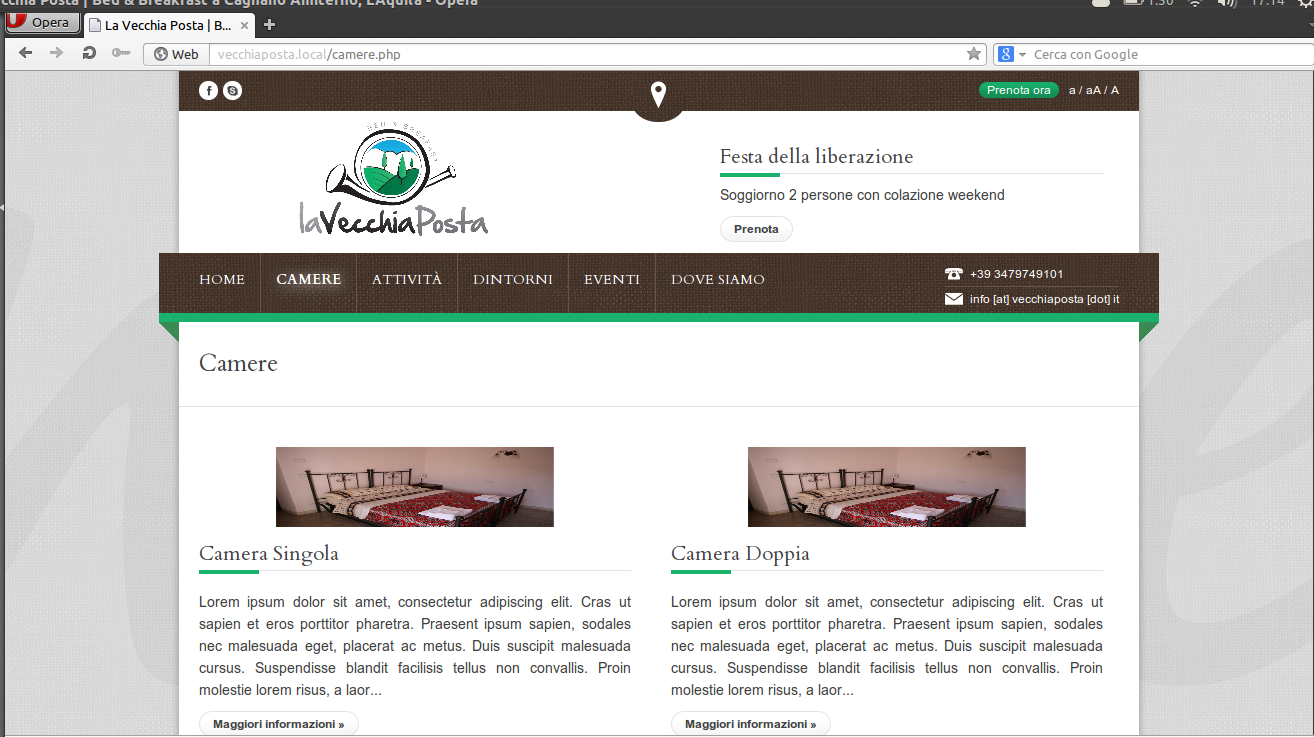
\includegraphics[width=0.9\textwidth,keepaspectratio=true]{../img/compOpera}
    \centering
    \caption{Compatibilità Opera}%
    \label{fig:compOpera}%
\end{figure}

\begin{figure}[h!]%
    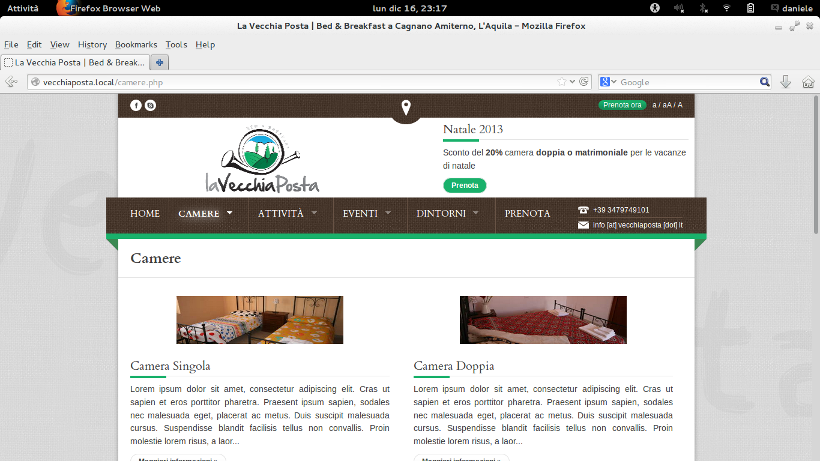
\includegraphics[width=0.9\textwidth,keepaspectratio=true]{../img/compFirefox}
    \centering
    \caption{Compatibilità Firefox}%
    \label{fig:compFirefox}%
\end{figure}

\begin{figure}[h!]%
    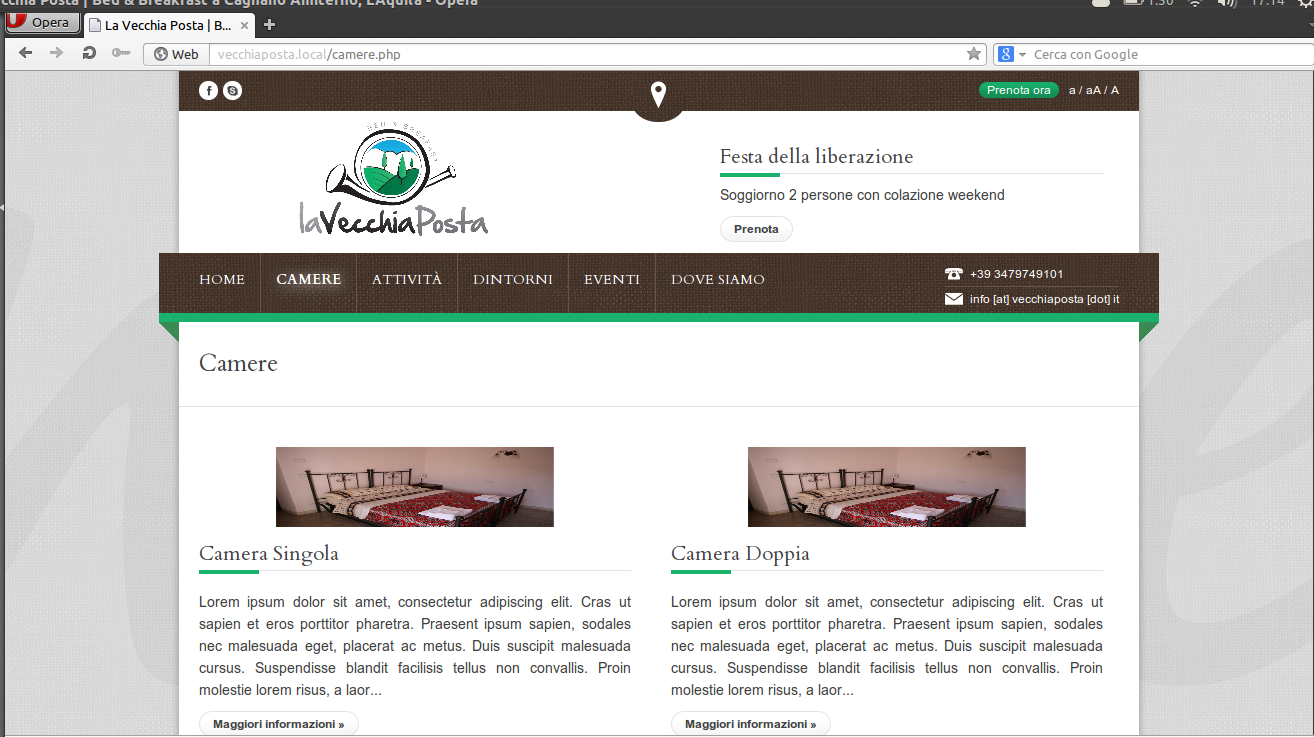
\includegraphics[width=0.9\textwidth,keepaspectratio=true]{../img/compOpera}
    \centering
    \caption{Compatibilità Opera}%
    \label{fig:compOpera}%
\end{figure}

\newpage
\section*{Utenti disabili}
Per quanto riguarda l'attenzione all'utilizzo dell'applicazione da utenti diversamente abili si posta l'attenzione al disfunzionalità del daltonismo, simulandone l'utilizzo 
tramite servizi offerti online. Si riporta uno screenshot di esempio.

\begin{figure}[h!]%
    
\includegraphics[width=0.9\textwidth,keepaspectratio=true]{../img/daltonismo}
    \centering
    \caption{Distorbo Protanopia}%
    \label{fig:daltonismo}%
\end{figure}
\par Non è stato l'unico test eseguito per testare la completa accessibilità dell'applicazione da utenti diversamente abili. Un altro test importante è stato testare l'applicazione
tramite un browser testuale, nel nostro caso si è utilizzato Lynx disponibile per linux. L'utilizzo di un browser testuale aiuta ad individuare eventuali dimenticanze nel campo alt per 
le immagini e mostra allo sviluppatore anche il corretto sviluppo dell'applicazione rispettando i canoni dettati dai motori di ricerca per i loro robots.

\begin{figure}[h!]%
    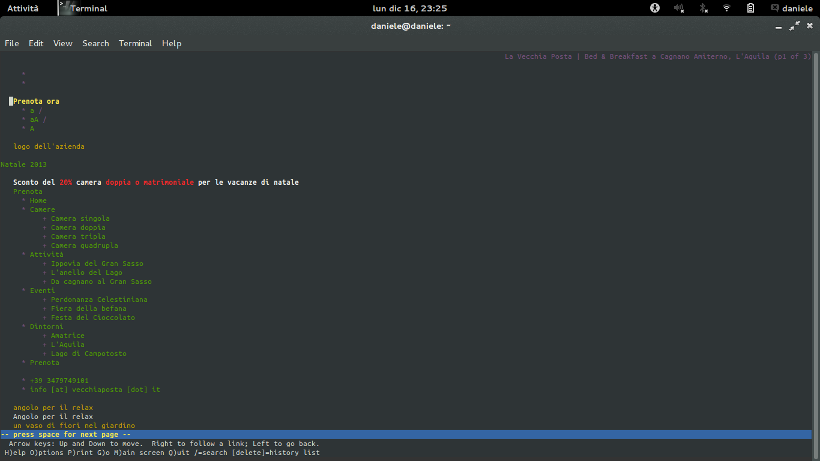
\includegraphics[width=0.9\textwidth,keepaspectratio=true]{../img/lynx}
    \centering
    \caption{Lynx scansione dell'applicazione}%
    \label{fig:lynx}%
\end{figure}

\newpage
\par Un ulteriore test per il check sull'accessibilità del sito è stato disabilitare il caricamento delle immagini e del javascript. Il risultato finale risulta essere non del 
tutto ottimale ma resta comunque accettabile l'accessibilità. Si riporta di seguito uno screenshot del test.
\begin{figure}[h!]%
    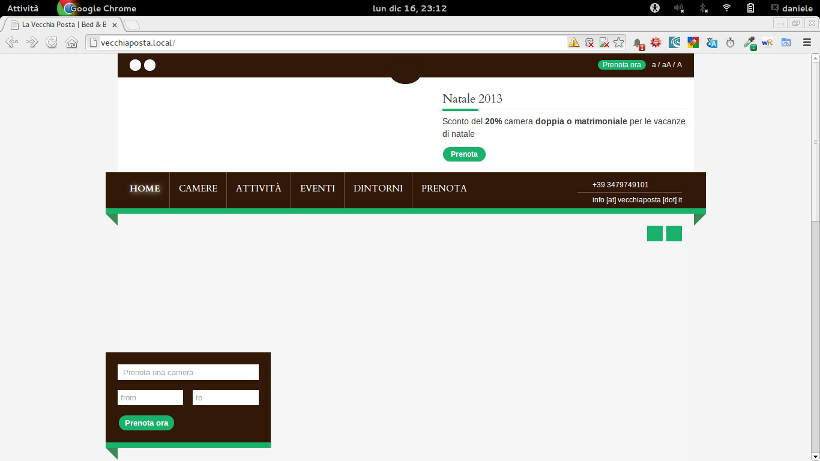
\includegraphics[width=0.9\textwidth,keepaspectratio=true]{../img/noJsNoImg}
    \centering
    \caption{Applicazione con Immagini e JavaScript bloccati}%
    \label{fig:noJsNoImg}%
\end{figure}

Per il test della luminostità abbiamo utilizzato la seguente formula:
\begin{center}
$\frac{(red*299)+(green*587)+(bluee*114)}{1000} \geq {125}$
\end{center}

tenstando la luminosità del menu, unico elemento ad avere del testo e un colore di sfondo differente dal bianco, il risultato è stato ottimo:
\\[1cm]
\begin{center}
$\frac{(49*299)+(24*587)+(7*114)}{1000} = 295$
\end{center}

Per testare la differenza tra il colore del testo e il colore dello sfondo si è eseguito il test rispettando l'equazione:
\begin{center}
$[max(red1,red2)-min(red1,red2)]+[max(green1,green2)-min(green1,green2)]+[max(blue1,blue2)-min(blue1,blue2)]\geq{500}$
\end{center}
ottenendo come risultato
\begin{center}
$[244-49]+[244-24]+[244-7]={652}$
\end{center}

\end{document}          